\documentclass{article}

\usepackage[frenchb]{babel}
\usepackage[T1]{fontenc}
\usepackage[utf8]{inputenc}
\usepackage{graphicx}
\usepackage[hypertexnames=false, pdftex]{hyperref}
\hypersetup{ colorlinks = true, linkcolor = black, urlcolor = blue, citecolor = blue }

\makeatletter
 
\newskip\@bigflushglue \@bigflushglue = -100pt plus 1fil
 
\def\bigcenter{\trivlist \bigcentering\item\relax}
\def\bigcentering{\let\\\@centercr\rightskip\@bigflushglue%
\leftskip\@bigflushglue
\parindent\z@\parfillskip\z@skip}
\def\endbigcenter{\endtrivlist}
 
\makeatother

\title{Diagrammes UML}
\author{Anthony Brunel et Antoine Laurent}

\date{\today}

\begin{document}
\maketitle
\newpage
\tableofcontents
\listoffigures
\newpage

\section{Introduction}

Ci-dessous les différents diagrammes UML demandés pour le projets.

\subsection{UML métier}

Pour le diagramme de classe, on a choisit une implémentation simple avec les classes tâche ponctuelle et au long cours qui héritent de tâche. 
On a choisis de créer une classe manager pour conserver les donées que ça soit les tâches ou les catégories.
On a aussi créé des énumérations pour les différents types et importances.

\subsection{UML graphique}
Pour la partie graphique on a essayé de respecter le model MVC, avec une classe pour chaque frame nécessaire et un controler qui va définir les actions a réaliser lorsqu'un listener est "activé".

\subsection{Javadoc}

On a fait une javadoc pour que notre projet soit plus simple à comprendre et à apréhender, vous pouvez la retrouver \href{run:../doc/index.html}{ici}

\clearpage
\section{Diagramme de classe métier}

\begin{figure}[h]
	\bigcentering	
	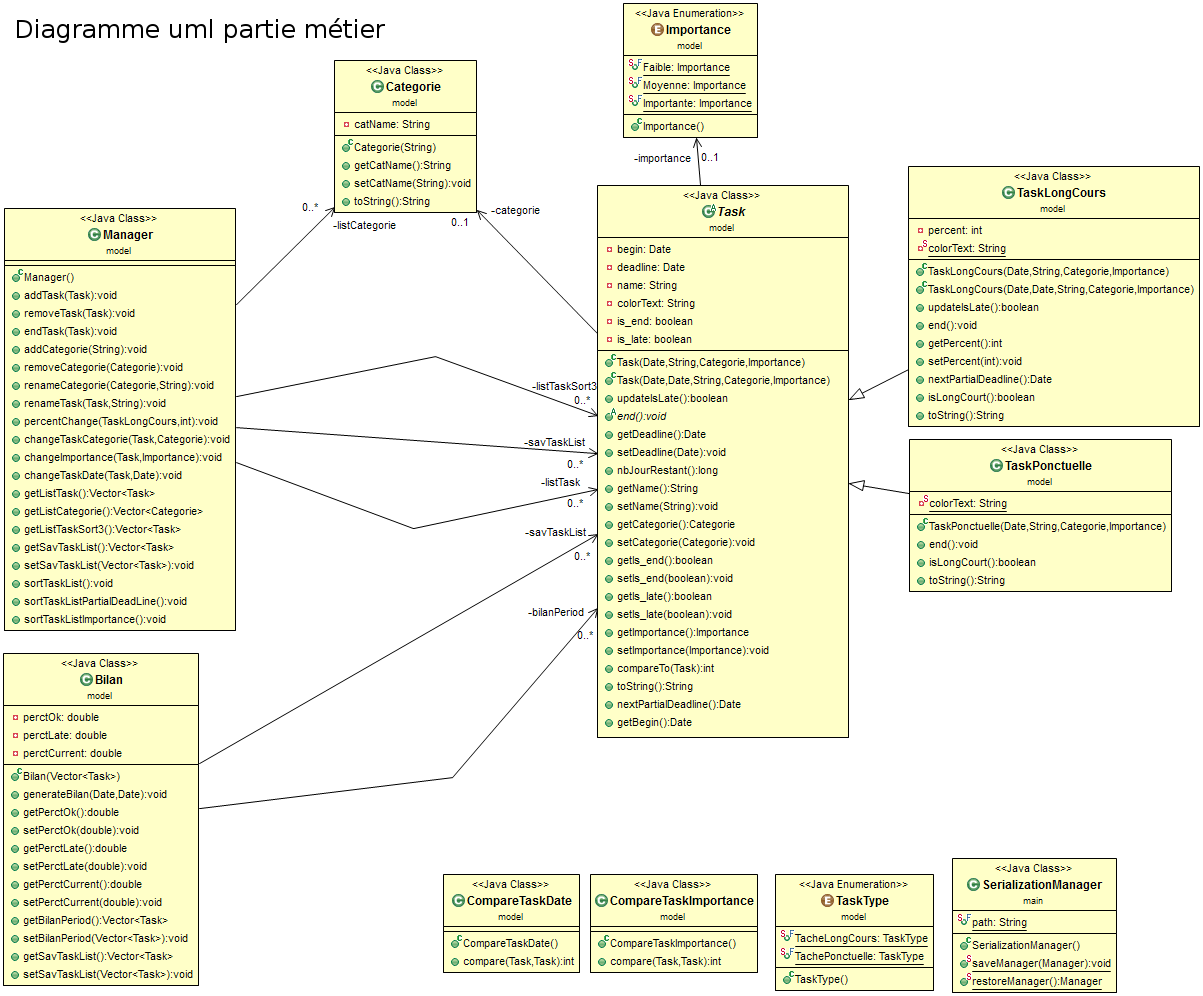
\includegraphics[scale=0.4]{UML/umlModel.png}
	\caption{UML métier}
	\label{UML metier}
\end{figure}

\clearpage

\section {Diagramme de classe graphique}

\begin{figure}[!h]
	\bigcentering	
	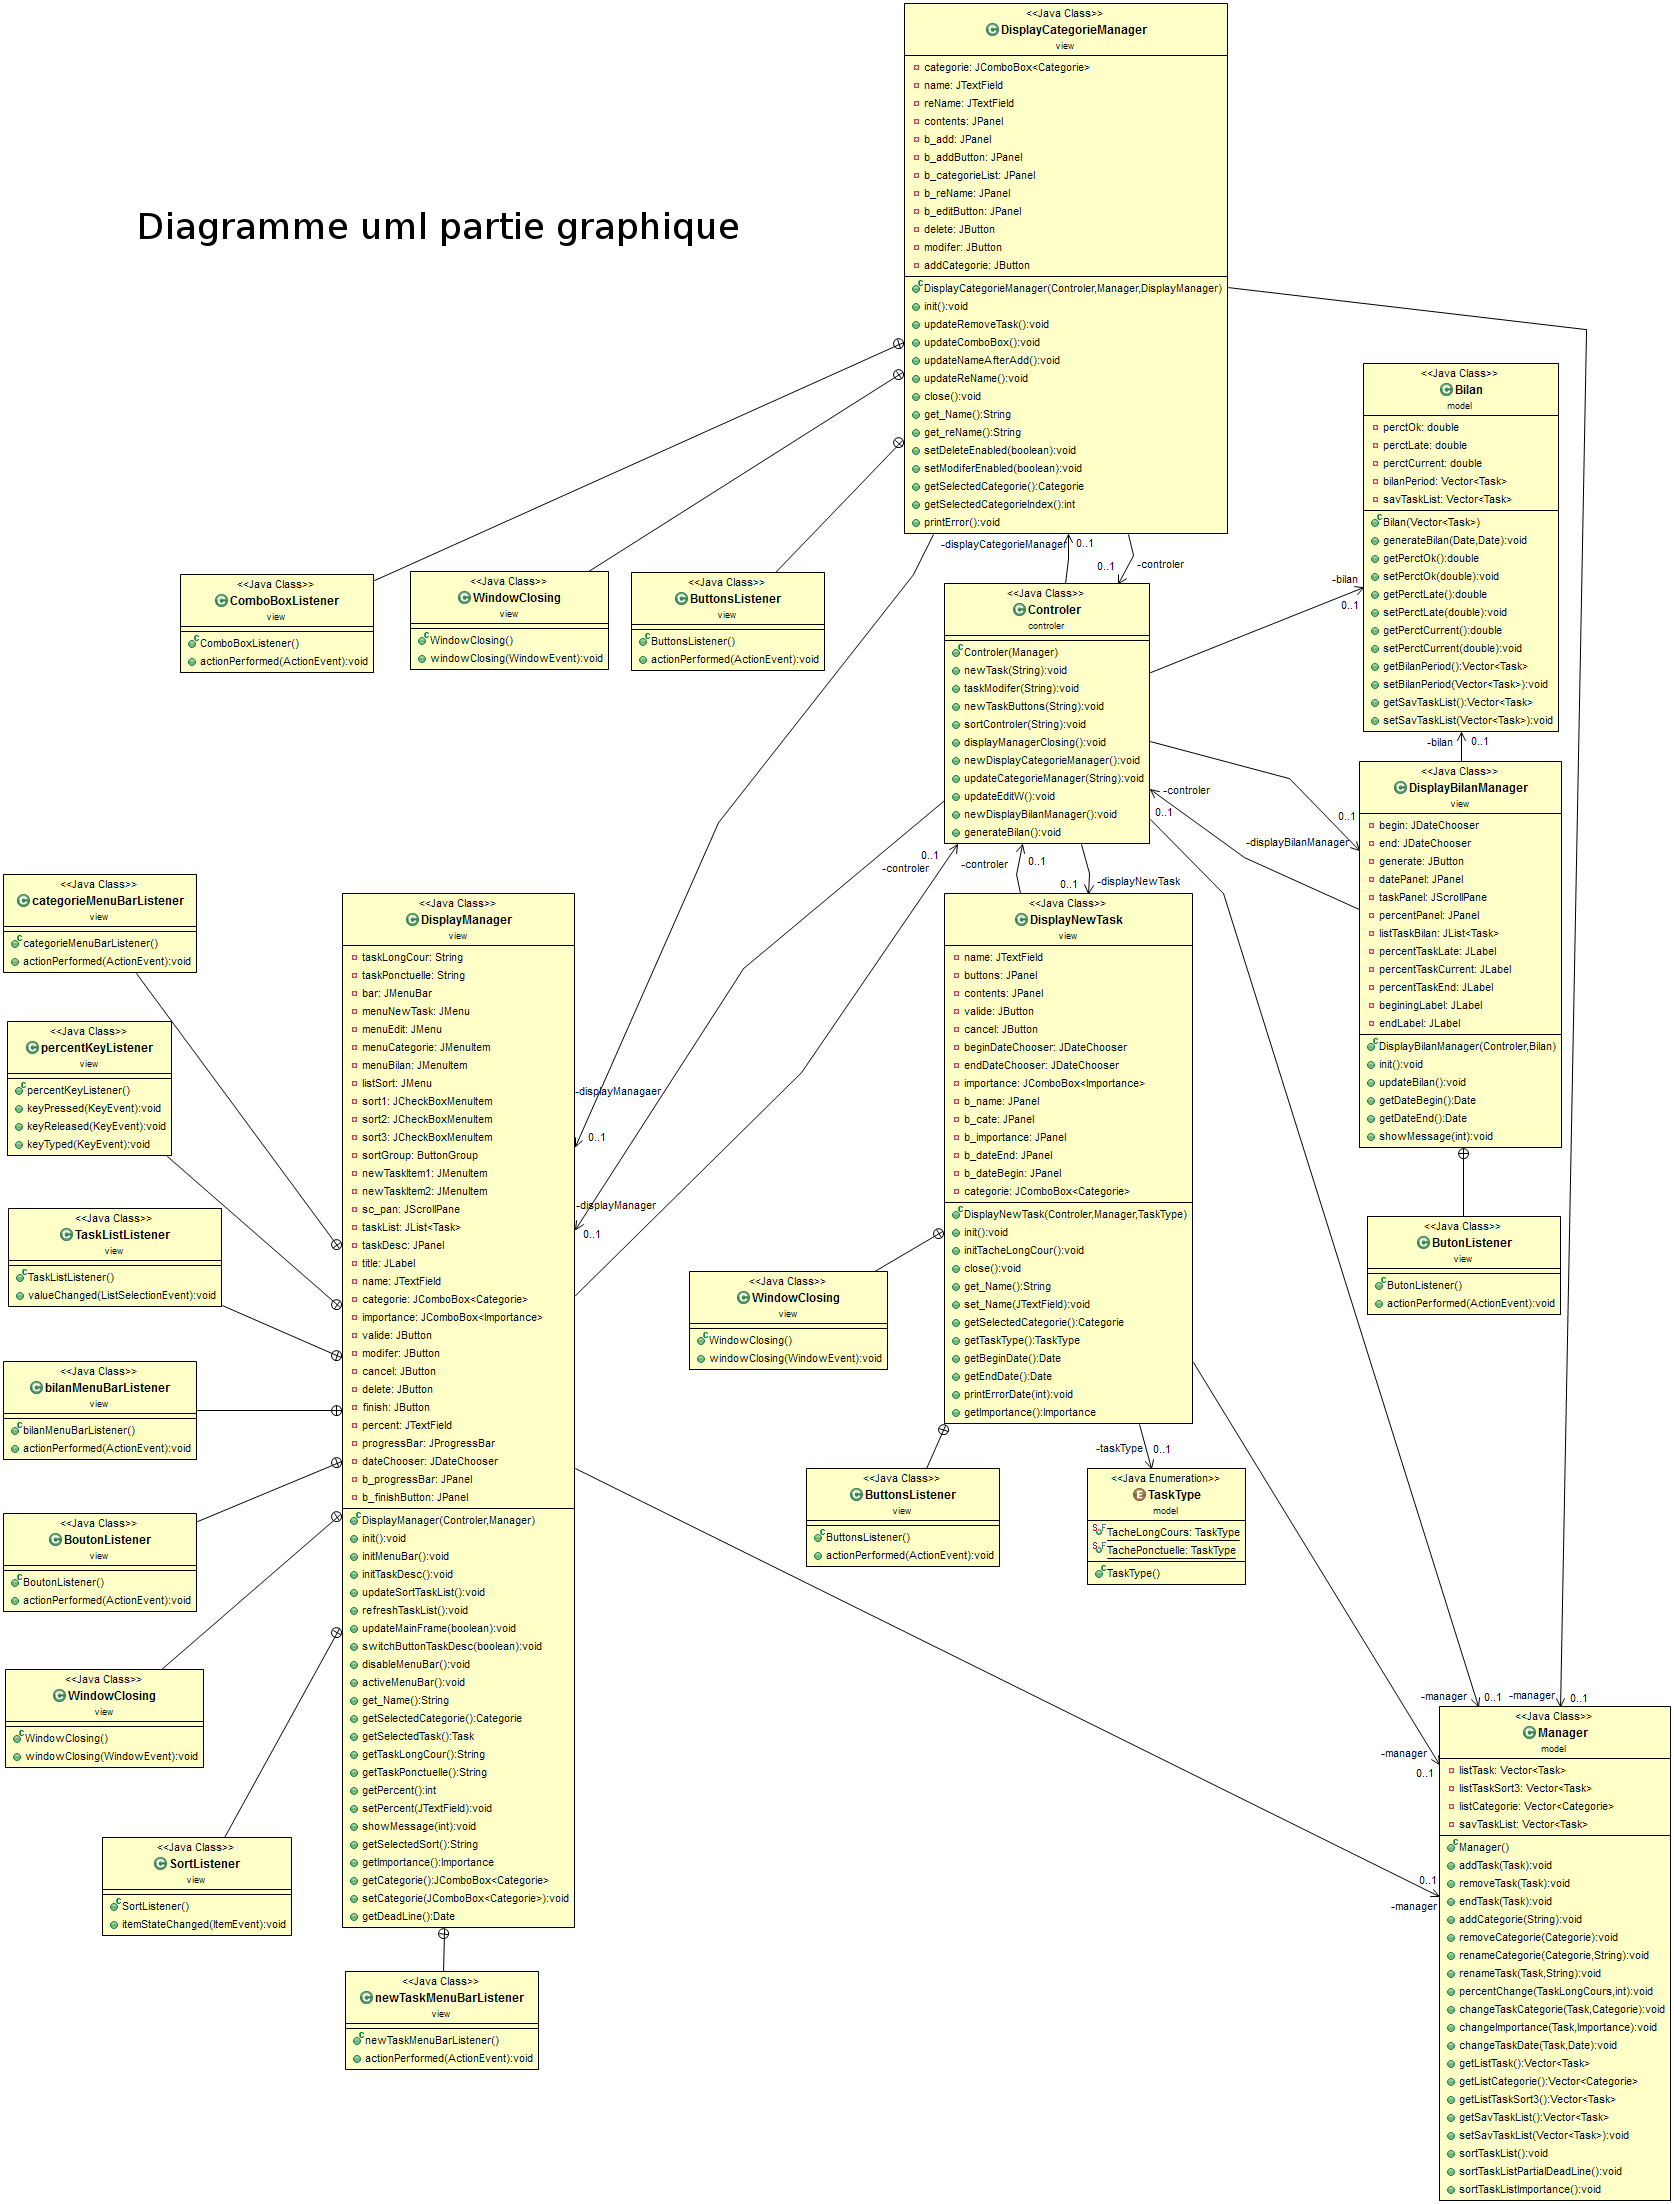
\includegraphics[scale=0.22]{UML/umlGraphic.png}
	\caption{UML graphique}
	\label{UML graphique}
\end{figure}

\section{Diagrammes état transitions}

\begin{figure}[!h]
	\bigcentering	
	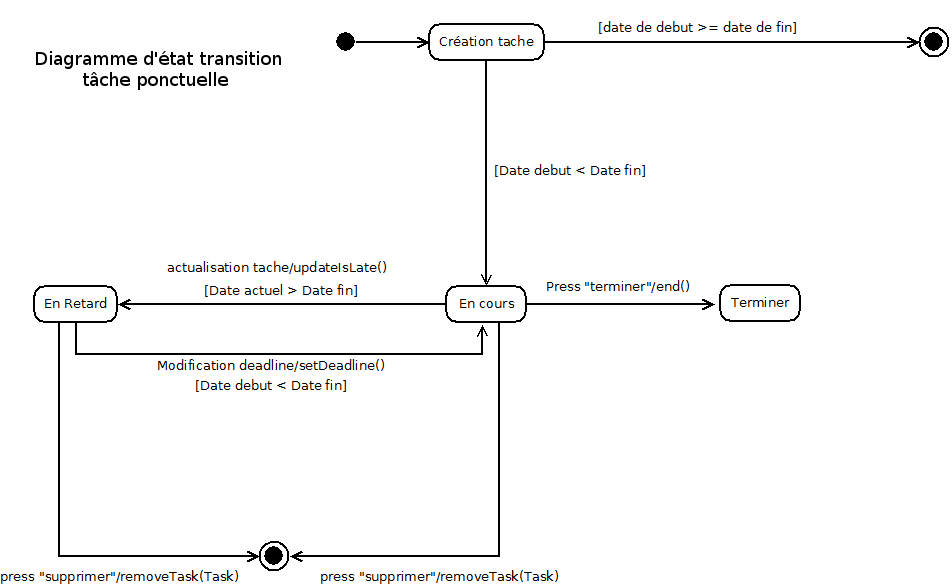
\includegraphics[scale=0.34]{UML/tache_ponctuelle.png}
	\caption{UML état transition tâche ponctuelle}
	\label{UML état transition tâche ponctuelle}
\end{figure}

\begin{figure}[!h]
	\bigcentering	
	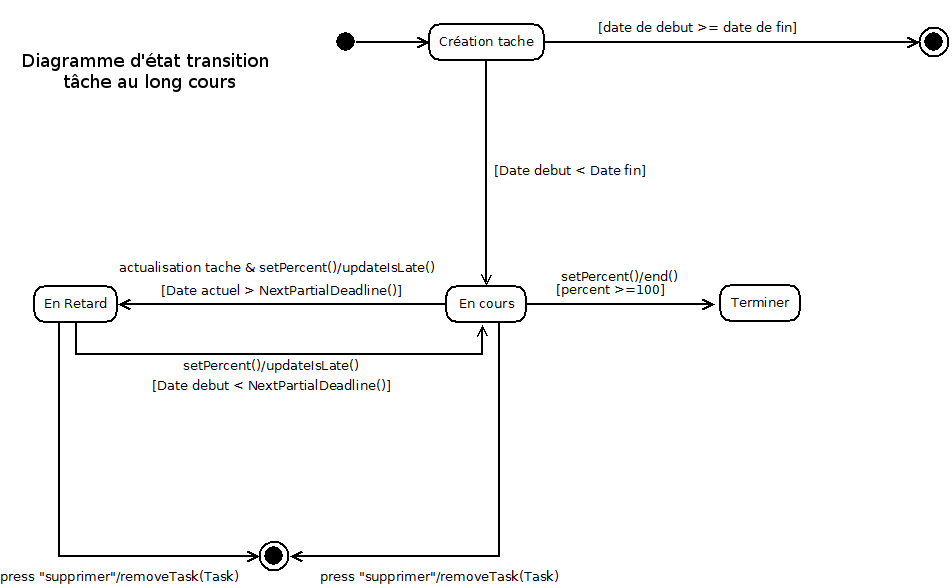
\includegraphics[scale=0.34]{UML/tache_long_cours.png}
	\caption{UML état transition tâche long cours}
	\label{UML état transition tâche long cours}
\end{figure}

\section{Diagramme de séquences}

\begin{figure}[!h]
	\centering	
	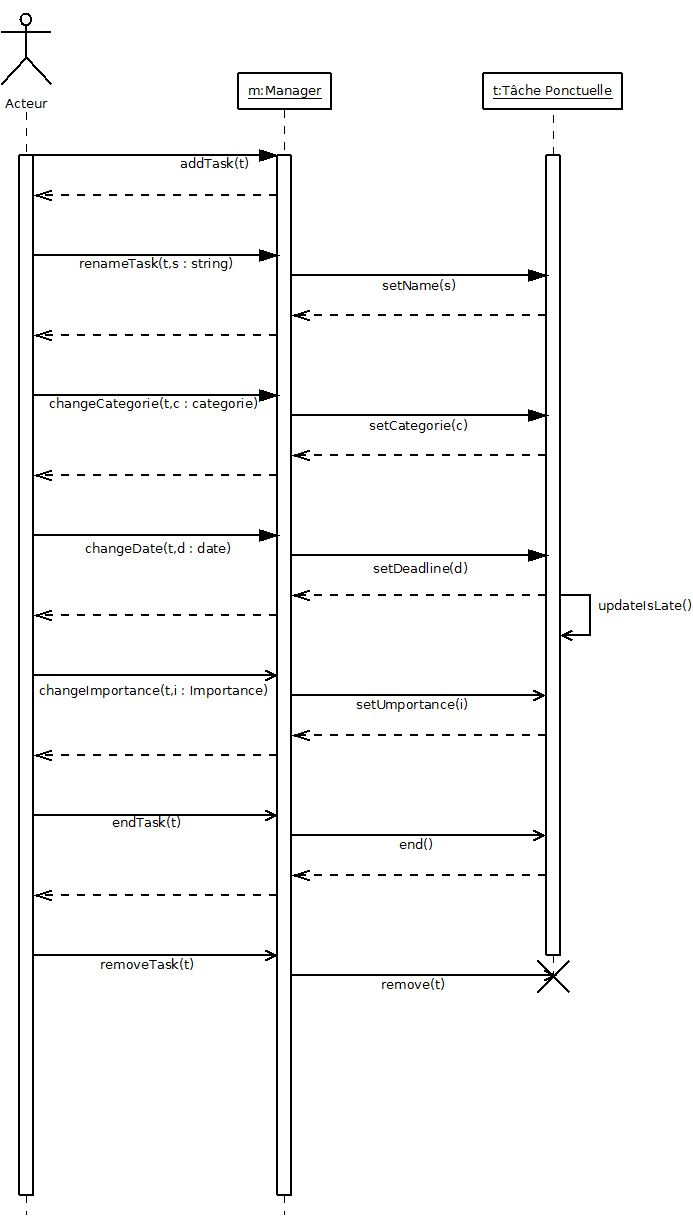
\includegraphics[scale=0.4]{UML/diagramme_de_sequence.png}
	\caption{UML séquence : utilisateur - tâche}
	\label{UML séquence : utilisateur - tâche}
\end{figure}

\end{document}
